\section{实现内核模块}
\subsection{参数传递}
本内核模块需要接收三个参数,一个 \texttt{int} 型的操作数,一个 \texttt{int} 数组,以及一个
\texttt{char*} 型的字符串表示当前的操作。因为 C array 没法获得长度,所以
还需要额外的一个 \texttt{int} 型的变量来表示数组的长度。

本处使用了 \texttt{module_param} 来读取非数组的参数,权限设置成0,使得
这些参数只能被内核模块自己修改。对于数组参数,使用了 \texttt{module_param_array},
该宏的原型是
\begin{lstlisting}[language=C]
#define module_param_array(name, type, nump, perm)		\
	module_param_array_named(name, name, type, nump, perm)

\end{lstlisting}

我们按照顺序,先传入数组,再传入类型(int),接着传入数组长度的参数,最后设置权限为0。

\subsection{内核模块的初始化}
本实验的要求是创建 \texttt{proc} 文件 \texttt{/proc/<ID>/calc},
因此需要先通过 \texttt{proc\_mkdir} 创建 \texttt{/proc/<ID>} 目录,如果本步骤无法完成,
那么释放proc资源,并且打Error log,然后返回。如果能够成功创建子目录,那么就可以通过
\texttt{proc_create} 创建 \texttt{calc} 文件,权限设置为0644,表示
内核可读写,但是其他均只能读。如果创建失败,那么释放之前分配的所有资源,然后打Error log,并且
返回。反之,则完成了初始化的工作。

\subsection{内核模块的清理}
一个成功初始化的该内核模块一共有两个资源,一个是 \texttt{proc} 文件,
一个是 \texttt{proc/<id>} 目录。先释放 \texttt{proc} 文件,然后释放目录,即完成了清理工作。

\subsection{内核模块的读}
实验要求是当用户读取文件时,输出以逗号分隔的数组结果。我的处理逻辑如下,
根据操作符的类型,在迭代数组的同时完成对应的操作,同时将结果转成字符串append至一个临时
数组中。在迭代完成后,将该数组从kernel拷贝到用户态,即完成了读的操作。

在完成的过程中有以下几点需要注意。

首先,因为kernel programming不允许使用常规头文件,我们需要使用 \texttt{strcpy}和
\texttt{snprintf}来完成字符串的比较和格式化拼接。所以我们该函数被
包含在了 \texttt{linux/string.h} 中,引用之即可。

其次,由于C string是以\texttt{backslash 0}作为结尾的,我们需要将格式化后的字符串数组的
最后一位设置为\texttt{backslash 0},以防用户读取出错。此外,由于数组的最后一个元素后无需
输出逗号,我们可以直接修改格式化数组的倒数第二位,将其从逗号改为\texttt{backslash n}。

\subsection{内核模块的写}
实验要求是当用户传入一个数字后,将其作为新的操作数。我的处理逻辑如下,
首先从用户态把buffer拷贝到kernel buffer之中,然后检查操作数是否
是一个合法的整数,如果是则将其赋值给操作数,否则返回错误。

本部分实现较为简单,只需要使用 \texttt{kstrtoint} 函数即可。其他的错误处理和一般
处理方法一致。

\subsection{实验截图}

\begin{figure}[!h]
	\centering
	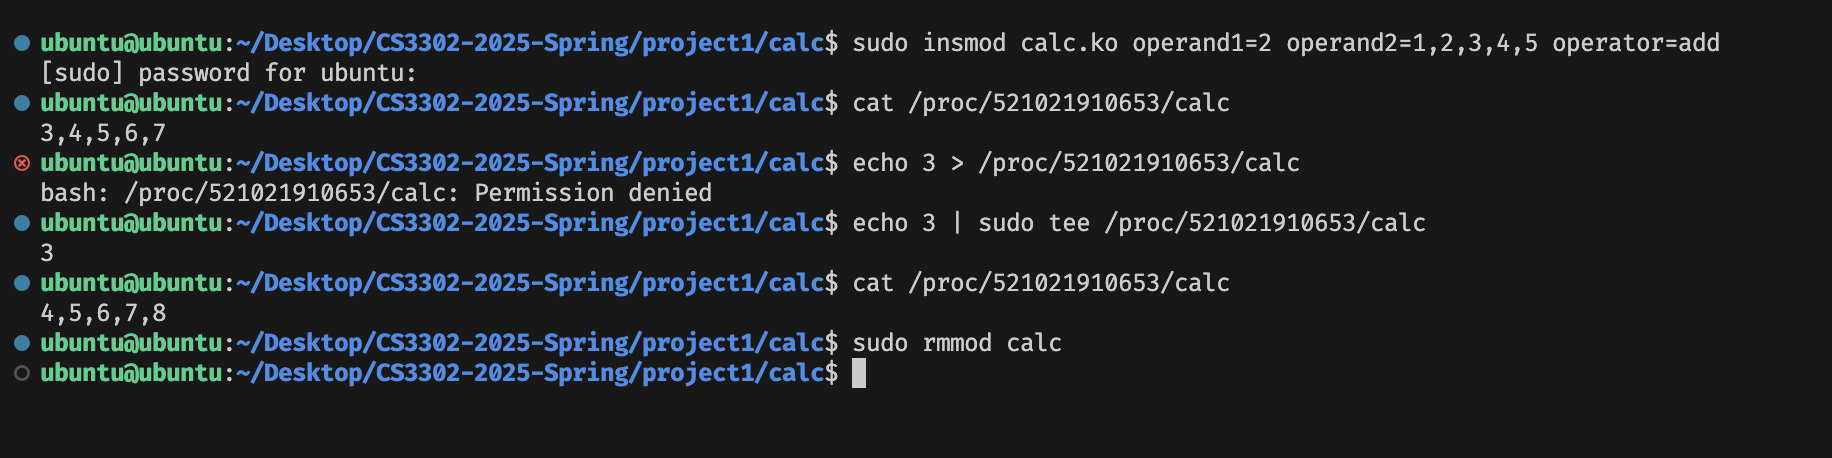
\includegraphics[width=0.8\textwidth]{../fig/add.png}
	\caption{Add操作截图}
\end{figure}

\begin{figure}[!h]
	\centering
	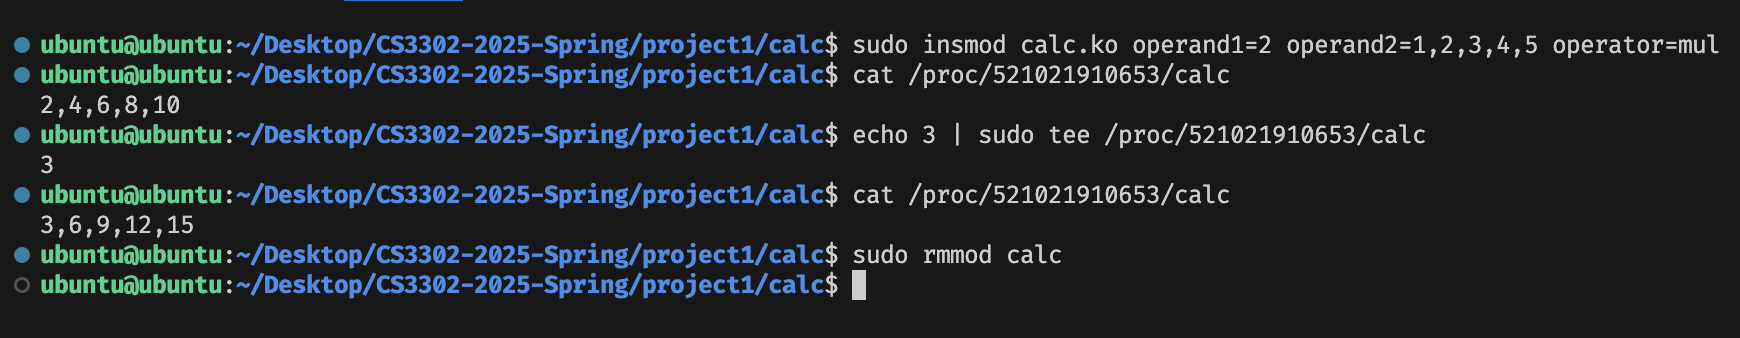
\includegraphics[width=0.8\textwidth]{../fig/mul.png}
	\caption{Mul操作截图}
\end{figure}

\subsection{实验心得}
本实验在完成的时候遇到了 \texttt{echo 3 > /proc/<id>/calc} 报权限不够的错,
说明重定向的时候没有权限写入,该问题是无法通过给echo加sudo权限解决的。
因此,我在写的时候,直接使用了 \texttt{echo 3 | sudo tee /proc/<id>/calc},
,tee是一个文件读写的操作,这样就可以成功写入了。

\section{实验用户态函数}

\subsection{解析进程状态}
本部分主要是解析\texttt{/proc/<id>/stat}文件,获得其进程状态信息。
通过\texttt{cat},我们可以发现该文件的第三个字段是进程状态,并且字段间
是以空格分隔的。因此,只需要写一个简单的循环,跳过前两个连续的字符串即找到了
目标状态信息。

\subsection{解析命令行参数}
本部分的大体逻辑是,首先检查\texttt{cmdline}文件是否非空,若为空,则去读取
\texttt{comm}文件。若不为空,那么将文件内的\textbf{所有}内容拷贝至传入的buffer之中。

我一开始是用\texttt{fgets}来读取文件,但是发现读取的内容不完整,因为读到\texttt{backslash n/0}就停止了。
并且通过\texttt{cat cmdline}的时候发现里面存在特殊字符\texttt{\textasciicircum @},经查阅得知这是\texttt{backslash 0}的含义,这更加证明了
不能使用\texttt{fgets}。

所以我后来改为使用\texttt{fread}来读取文件,将二进制比特全部拷贝到buffer之中。
在拷贝完成之后,还需要遍历一边buffer,将\texttt{\textasciicircum @}替换为\texttt{space},这样就完成了解析。如果不这么做,
用户在输出的时候仍然只能输出部分的cmdline信息。

针对\texttt{comm}文件的读取与上述类似,不再赘述。

\subsection{main函数}
main函数里主要就是调用上述实现的两个函数,非常简单。

值得一提的是\texttt{pid}的获取,因为main函数里\texttt{pid}的buffer只有16字节的长度,而
\texttt{dirent}里的\texttt{d\_name}最大长度是256字节,单纯使用
\texttt{strncpy/snprintf}都涉及到truncate的问题,而无法通过编译。
为此我修改了makefile,添加了\texttt{-Wno-stringop-truncation}来关闭这个warning。

\subsection{实验截图}

\begin{figure}[!h]
	\centering
	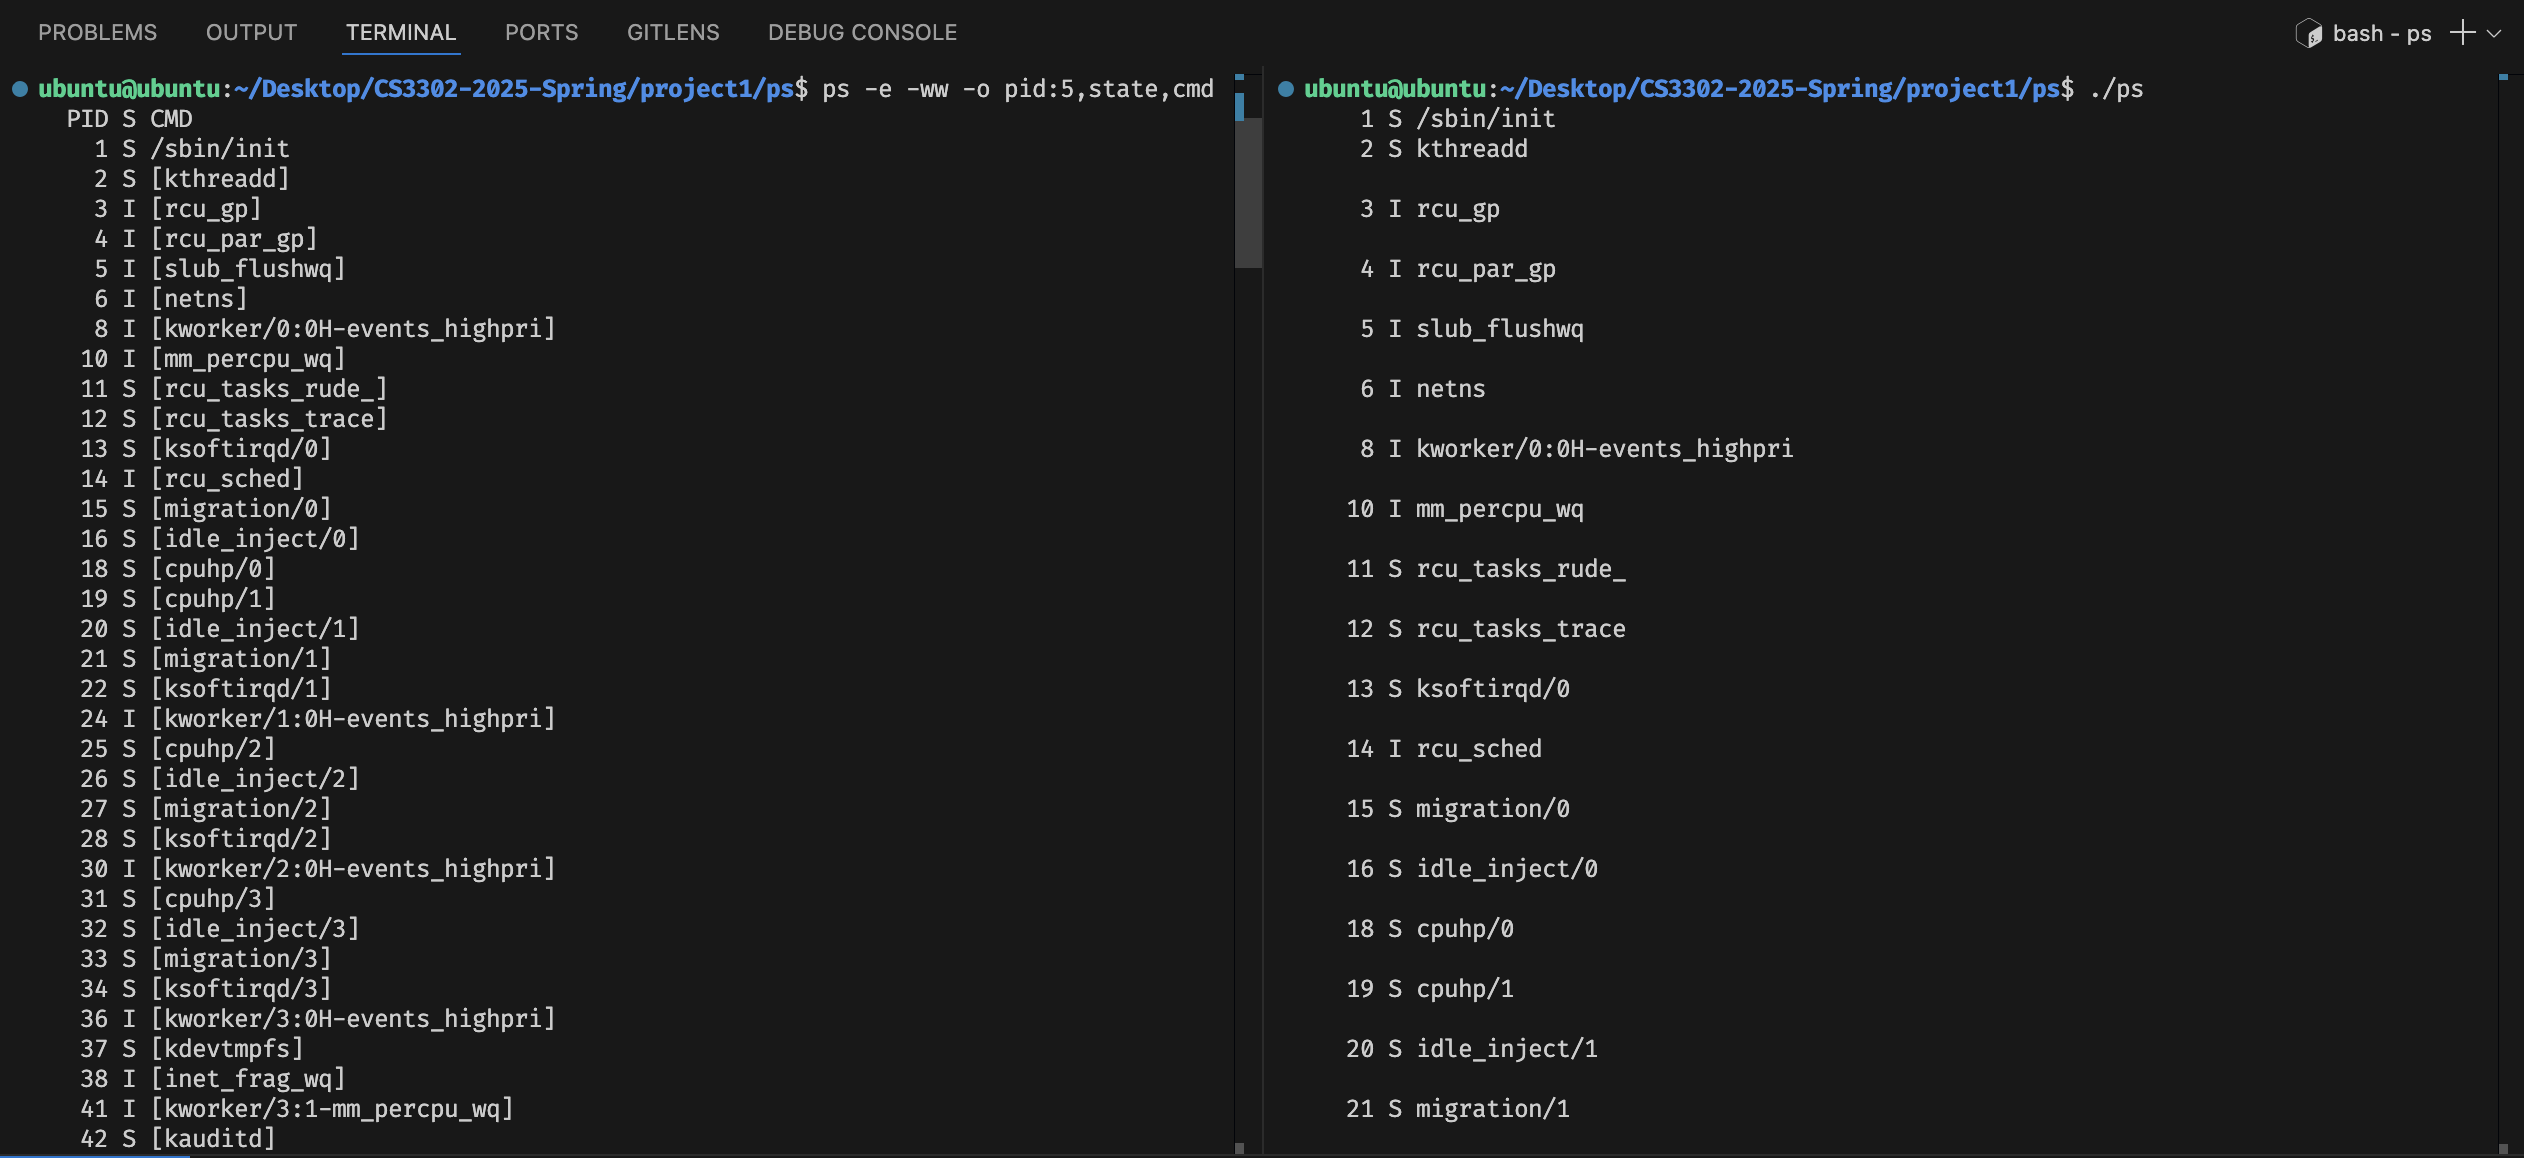
\includegraphics[width=0.6\textwidth]{../fig/p1.png}
	\caption{截图1}
\end{figure}

\begin{figure}[!h]
	\centering
	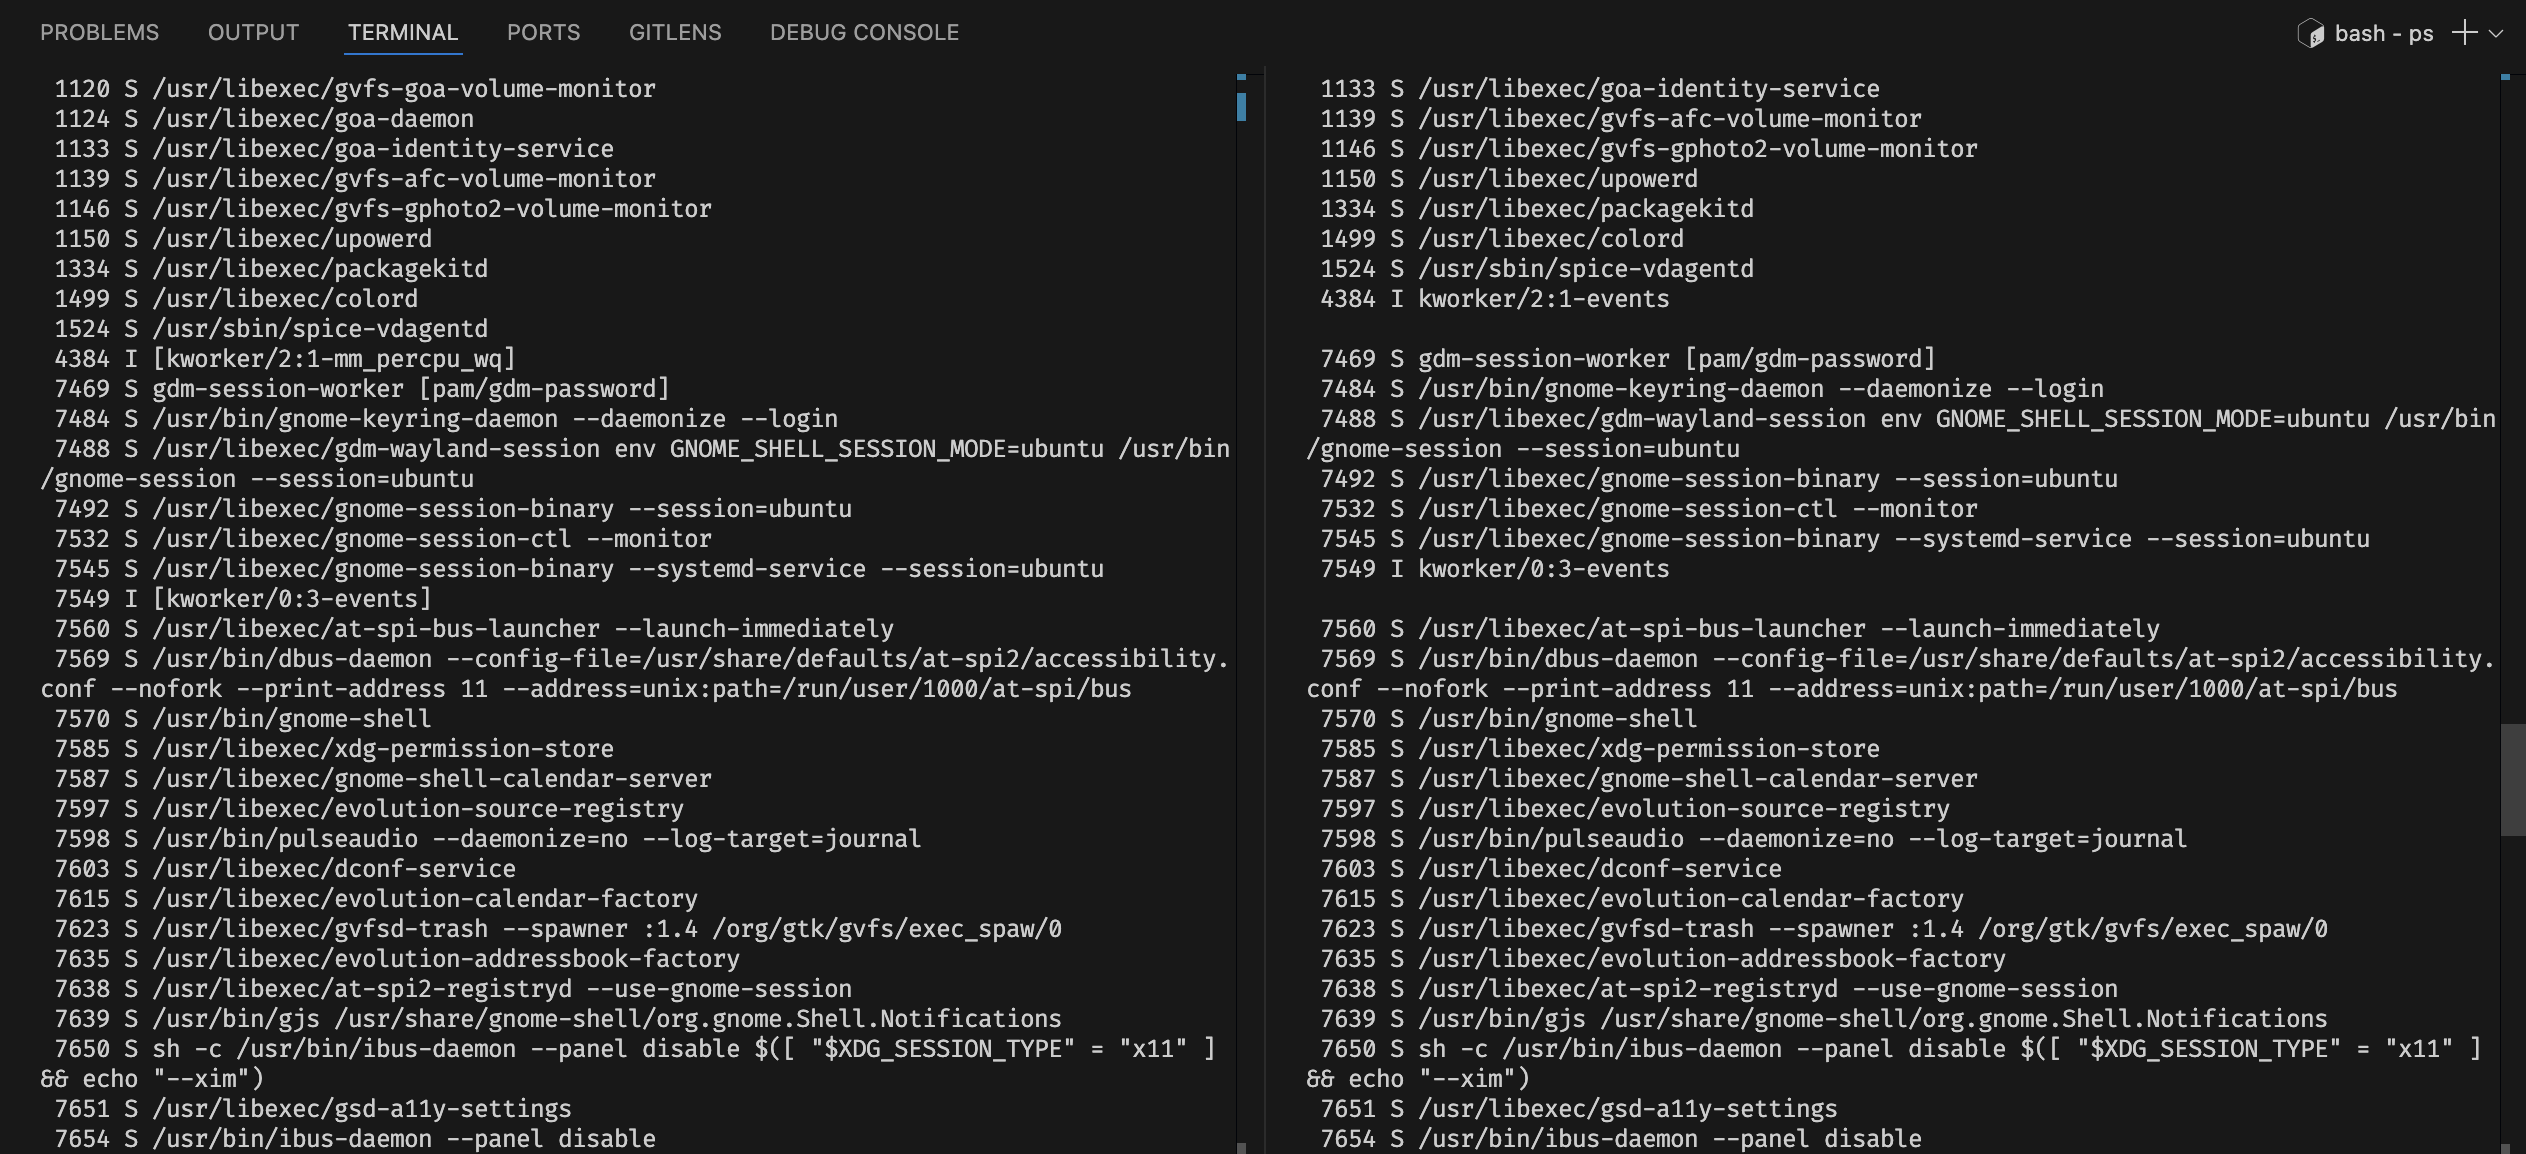
\includegraphics[width=0.8\textwidth]{../fig/p2.png}
	\caption{截图2}
\end{figure}

\section{实验心得}
经过本次实验,我了解如何编写内核模块,并且通过kernel提供的接口完成
kernel和用户态的交互;也学会了以用户态的身份去获取部分内核信息。这是
对庞大linux内核的一个很好的入门,也是对操作系统的一个很好的实践。

我的实验代码开源在 
\href{https://github.com/JackeyHua-SJTU/linux-kernel}{GitHub}上。